

Le programme MASTA est une simulation multi-agents d'allocation de
tâches pour la récolte de ressources. 

\section{Le monde}

Le monde de Masta est composé d'agents humains qui doivent récolter
différentes ressources pour le compte de l'agent hutte à laquelle ils sont
rattachés. Ces ressources sont de trois types : viande, baies,
bois. Les baies et le bois sont représenter par une variable
de \og{}patch\fg{}, la viande peut être récupérée sur un agent mouton mort. 


\section{Les agents humains}

Les agents humains sont tous rattachés à une hutte qui s'occupe de
leur allouer leurs tâches. Leur couleur représente leur tâches actuel,
rouge pour chasseur, vert pour cueilleur, jaune pour bûcheron. Un
humain effectue sa tâches jusqu'à avoir récolter une quantité préfixé
de ressource puis, une fois cette quantité atteinte, il rentre à sa
hutte où il se verra allouer une nouvelle tâches. {\bf Plus un
humain effectue une tâche plus il est performant dans celle-ci}.

\section{Les huttes}

Les huttes jouent un rôle crucial dans Masta. Elles organisent la
répartition des tâches entre les agents humains. Le but pour
chaque hutte est de récolter le maximum de ressources possibles de
façon la mieux répartie possible. Trois types de huttes ont été
implémenter, représentant chacun un type d'allocation différents.

\begin{minipage}[H]{0.1\linewidth}
  \begin{figure}[H]
    \begin{center}
      
\includegraphics[width=0.5\textwidth]{./img/hut_static}
    \end{center}
  \end{figure}
\end{minipage}
\begin{minipage}[H]{0.9\linewidth}
  Les huttes de type \og{}static\fg{} allouent une tâche à chaque agent
  humain à la création de celui-ci puis lui réalloueront toujours cette même tâche.
\end{minipage}

\begin{minipage}[H]{0.1\linewidth}
  \begin{figure}[H]
    \begin{center}
      
\includegraphics[width=0.5\textwidth]{./img/hut_min_before}
    \end{center}
  \end{figure}
\end{minipage}
\begin{minipage}[H]{0.9\linewidth}
  Les huttes de type \og{}min before\fg{} allouent toujours la tâche
  correspondant à la ressource qui est actuellement au niveau le plus faible.
\end{minipage}

\begin{minipage}[H]{0.1\linewidth}
  \begin{figure}[H]
    \begin{center}
      
\includegraphics[width=0.5\textwidth]{./img/hut_affinity}
    \end{center}
  \end{figure}
\end{minipage}
\begin{minipage}[H]{0.9\linewidth}
  Les huttes de types \og{}affinity\fg{} allouent les tâches en
  fonction du niveau des ressources mais aussi en fonction des
  spécificités des agents. Ainsi un agent doué en chasse à plus de
  probabilité de se voir allouer cette tâche.
\end{minipage}

\section{Diagramme de classe}
  \begin{figure}[H]
    \begin{center}
      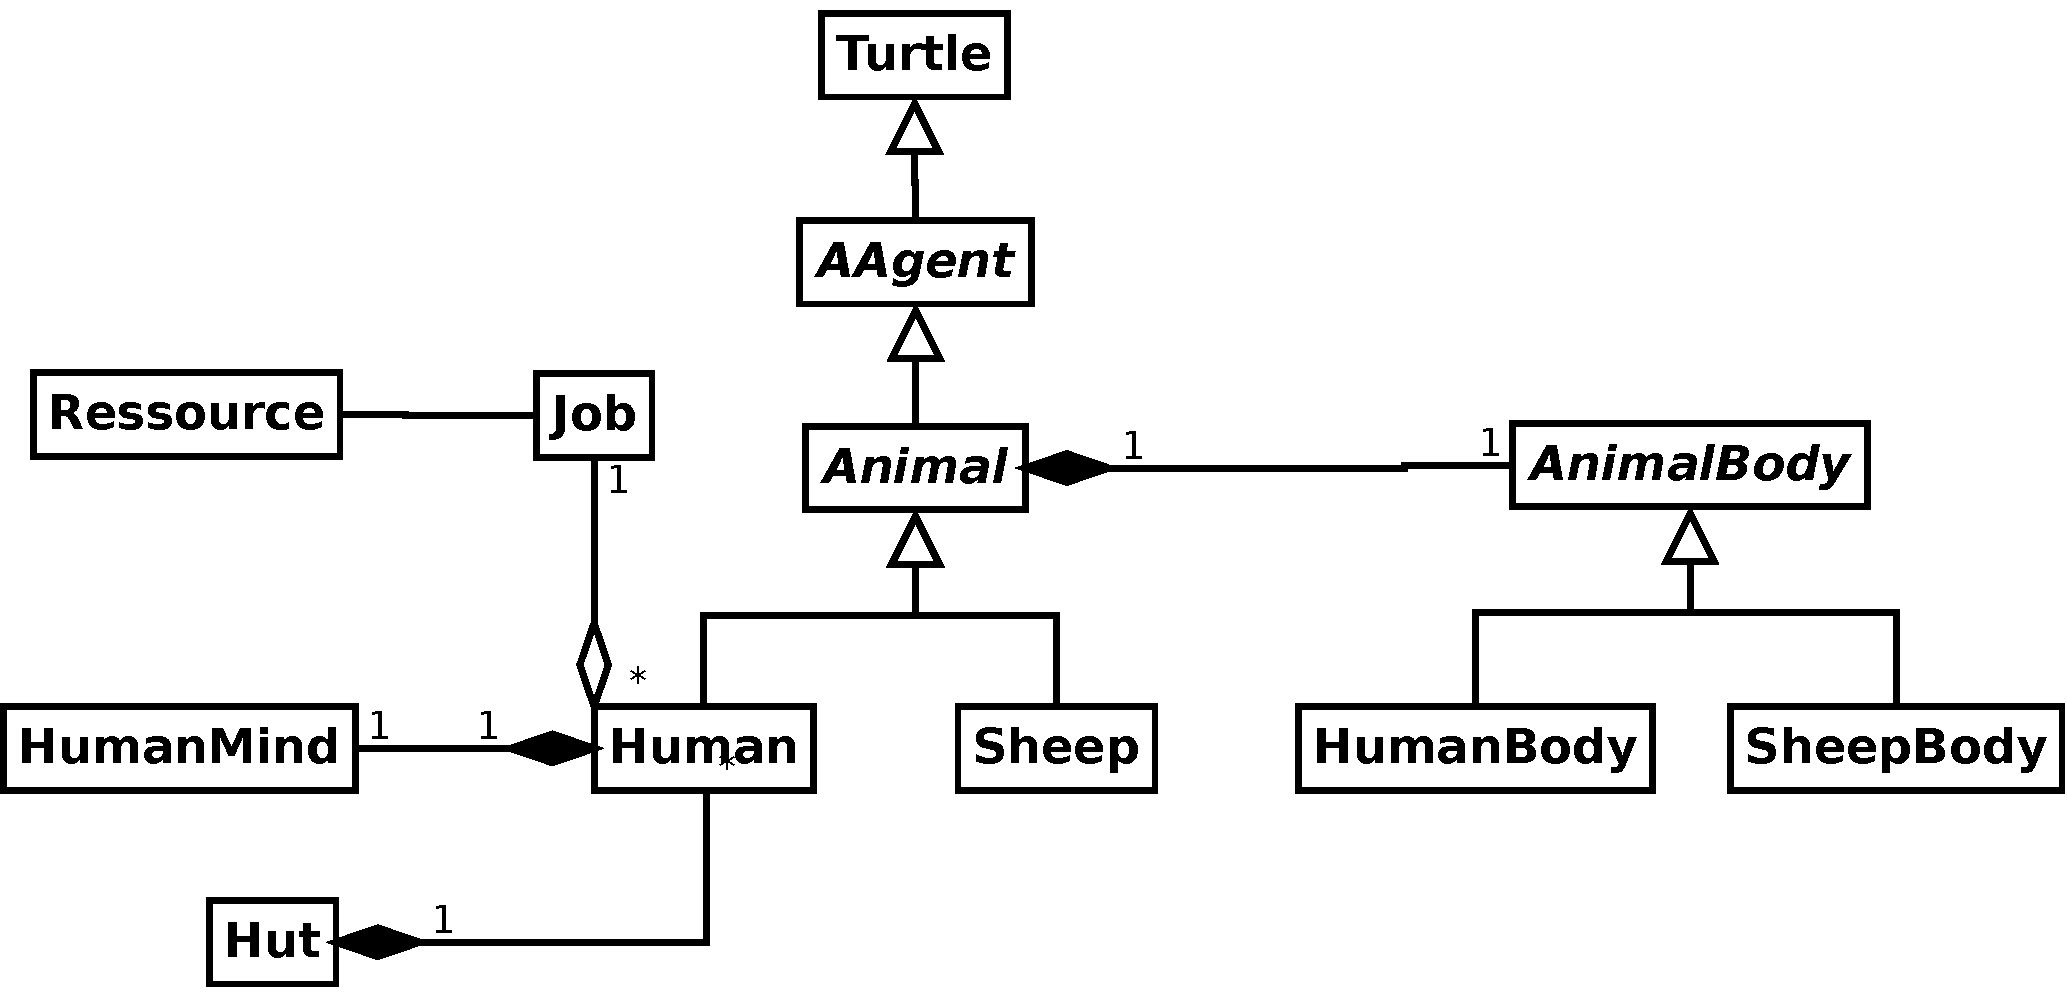
\includegraphics[width=0.6\textwidth]{./diags/uml}
    \end{center}
  \end{figure}
\section{Aperçu}

  \begin{figure}[H]
    \begin{center}
      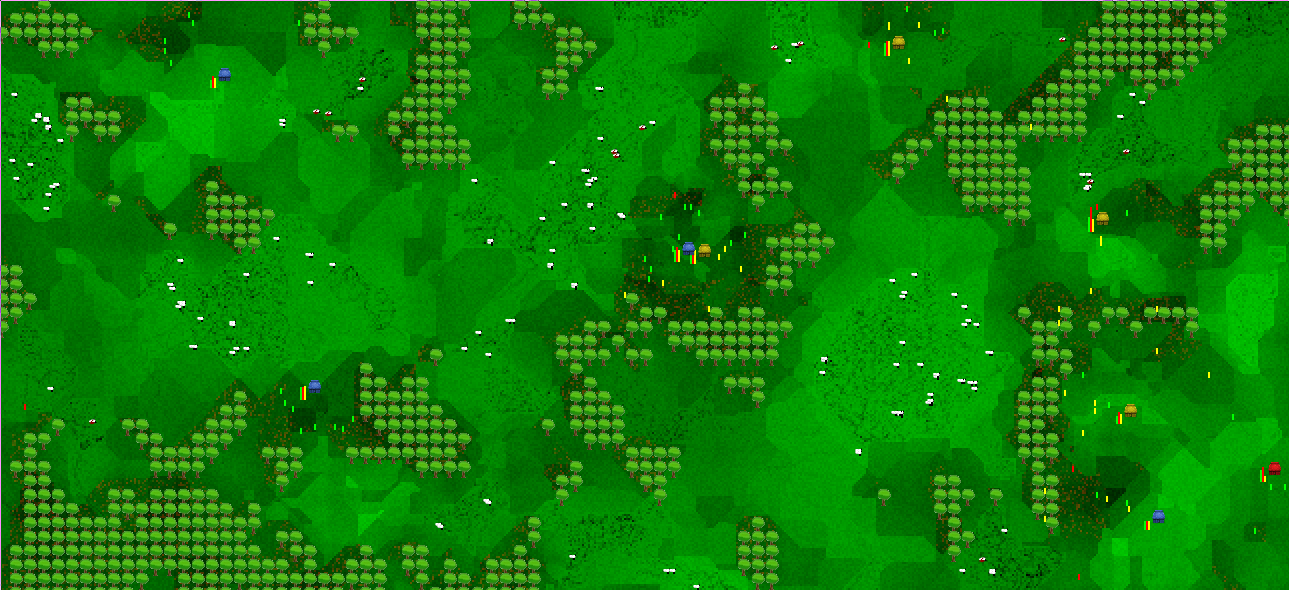
\includegraphics[width=0.75\textwidth]{./img/monde1}
      \caption{Aperçu globale}
    \end{center}
  \end{figure}

  \begin{figure}[H]
    \begin{center}
      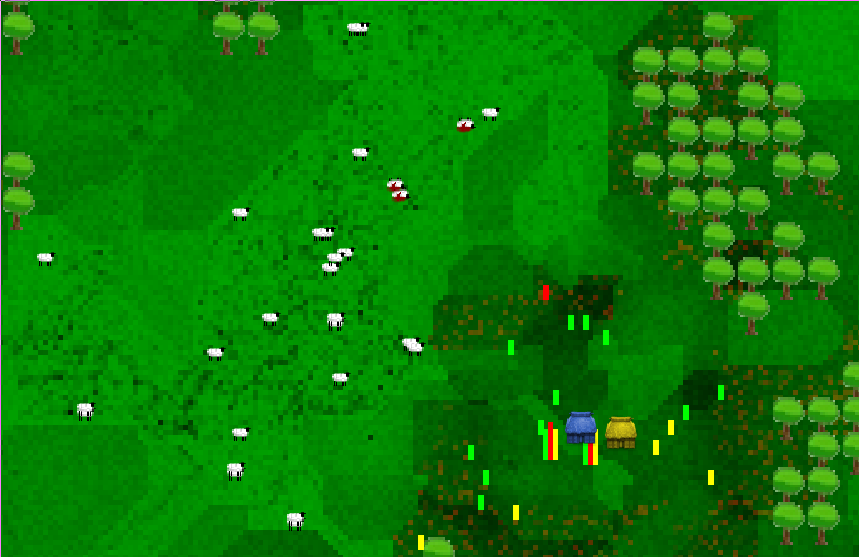
\includegraphics[width=0.6\textwidth]{./img/monde2}
      \caption{Aperçu zoomé}
    \end{center}
  \end{figure}

\section{Résultats}

  \begin{figure}[H]
    \begin{center}
      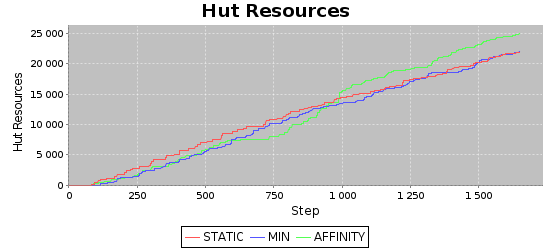
\includegraphics[width=0.6\textwidth]{./img/graph_ressources}
      \caption{Quantité de ressources récoltés par type de huttes en
    fonction du temps} 
      \label{fig:resultat}
    \end{center}
  \end{figure}

  Le graphique de la figure \vref{fig:resultat} représente la somme des quantités
  de la ressource de niveau minimal de chaque hutte pour chaque type
  de hutte en fonction du temps. Nous pouvons constater que les huttes
  de types \og{}affinity\fg{} (ici en vert) s'en sorte mieux, à long
  terme, que leurs homologues \og{}static\fg{} et \og{}min
  before\fg{}.

\section{Installation}

Cette application utilise TurtleKit et a était testé avec TurtleKit
2.4.8 actuellement disponible à l'adresse suivante :
http://gforge-lirmm.lirmm.fr/gf/download/frsrelease/138/1158/Tk2.4.8.Eclipse.zip

\begin{enumerate}
\item Télécharger TurtleKit, le dossier Tk2 est un projet
eclipse. {\bf Importez} le dans eclipse (testé avec eclipse 4.2.1).
\item Télécharger Masta
\item Placer le contenu du dossier source (src) de Masta dans le
dossier source (Tk2/src) de TurtleKit.
\item Exécuter le projet Tk2, en cas de besoin voici les paramètres \\
main class = madkit.boot.Madkit \\
arguments = madkit.kernel.Booter --graphics --config turtlekit2.cfg
-Xmx4G \\
\item Une fois TurtleKit lancé : Simulation -> Quick load ->
[\ldots]/masta/Masta.xml
\end{enumerate}
  